\documentclass[a4paper, 12pt]{article}
\usepackage{graphicx}
\usepackage{enumitem}
\usepackage{mathtools}
\usepackage{hyperref}
\usepackage{caption}
\usepackage{subcaption}
\def\code#1{\texttt{#1}}
\def\f#1{Figure \ref{fig:#1}}
\begin{document}

\title{\vspace{4.0cm}Applied GPU Programming - Assignment III\\
\large DD2360 HT20}
\author{Pontus Asp}
\date{\today}
\maketitle
\thispagestyle{empty}
\pagenumbering{roman}
\newpage

\clearpage
\pagenumbering{arabic}

% Write here ->
\section{Git repository}
I uploaded my git repository to GitHub. I use the same git repository for the entire course but the folder structure requested is still followed under the root folder. I also have 2 extra directories, one for this report and one where I have code from tutorials.
\\\\
Here is the link to my git repository:\\
\url{https://github.com/pontusasp/kth-dd2360/tree/master/Assignment_3}


% 1. Explain how the mapping of GPU thread and thread blocks (which is already implemented for you in the code) is working.

% 2. Explain why shared memory can (theoretically) improve performance.

% 3. Explain why the resulting image looks like a "grid" when the kernel is simply copying in pixels to the shared block. Explain how this is solved and what are the cases.

% 4. There are several images of different sizes in the image folder. Try running the program on them and report how their execution time relates to file sizes.
\section{Exercise 1}
% 1
In the code we were given, the kernel functions are called with the mappings like: \code{kernel<<<grid, block>>>(...)}. 

The \code{grid} variable is defined as a 2D grid where each axis corresponds to the number of threads in that "direction", in the x-axis we set the grid to have the same number of threads as the width of the input image, and in the y-axis we set the grid to have the same number of threads as the height of the input image.

The grid is also divided into blocks where a number of threads will be grouped together, and the \code{block} variable defines the dimension of this grouping. If we for instance have a grid with the size of 2000x1000 and a block size of 50x100 then the grid will get a structure of blocks like 40x100. All threads in a block will be executed on the same SM, and each SM also has a shared memory that each block can allocate memory on, which we utilize in the exercise.

% 2
Theoretically we should be able to increase performance with this shared memory since it is stored closer to the SM than the global memory that we would otherwise need to use. We also avoid using up more memory bandwidth to the global memory by utilizing the shared memory.

% 3
After we first implemented shared memory our image output looked like a grid. The explanation for this is that when we first added our shared memory we only copied the pixels "in range" of our block, i.e. a 16x16 grid of pixels. but the problem is that the filter we wanted to apply relied on looking on nearby pixels to decide the new color of the pixel we applied the filter on. So when we applied the filter on the border of our block we accessed pixels that we did not copy - so those pixels looked black to the filter and got applied to the pixel we were currently updating. I fixed this by making the last two threads in each row and column copy an extra pixel and placing it 2 pixels away in their individual direction. But, this does have an edge case where the pixels will not get copied in a 2x2 square where the two other problematic rows and columns intersect. I solved this by having the threads handling these intersecting rows and columns of pixels also copy a third pixel 2 steps diagonally from their own pixel. See \f{shared_memory} for a visual example.

% 4
When running the program with all the different images it seems to be the case that the time it takes to finish correlates linearly to the size of the images, which, is not weird since the work needed to be done also grows linearly with the size of the image.

\begin{figure}
    \centering
    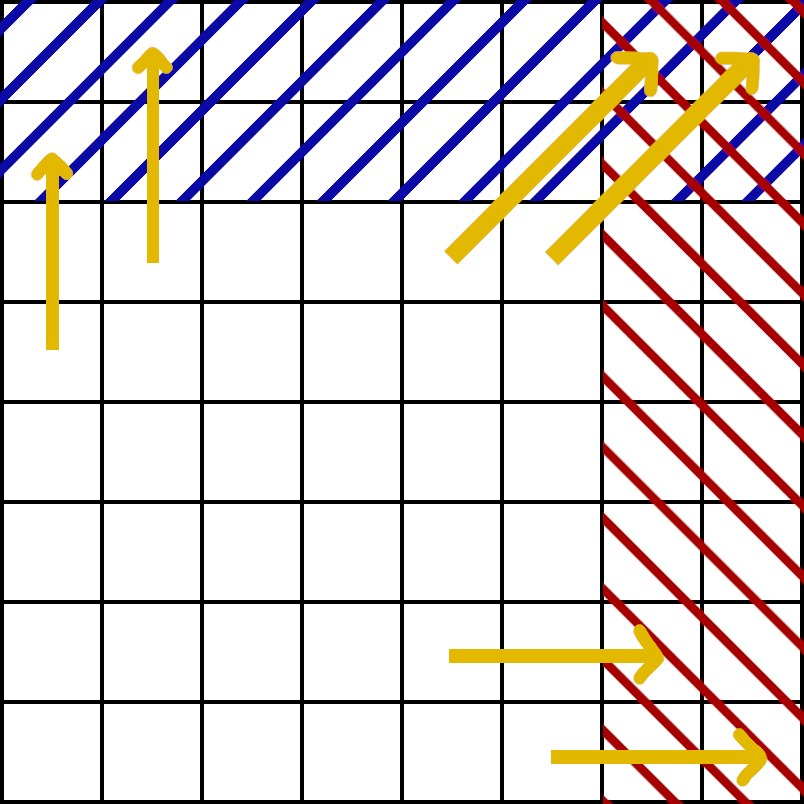
\includegraphics[width=0.5\linewidth]{images/shared_memory.png}
    \caption{Visual example of copying pixels to shared memory.}
    \label{fig:shared_memory}
\end{figure}


% 1. What are the differences between pageable memory and pinned memory, what are the tradeoffs?

% 2. Do you see any difference in terms of break down of execution time after changing to pinned memory from pageable memory?

% 3. What is a managed memory? What are the implications of using managed memory?

% 4. If you are using Tegner or lab computers, the use of managed memory will result in an implicit memory copy before CUDA kernel launch. Why is that?
\section{Exercise 2}
% 1
The difference between pageable memory and pinned memory is essentially that the pinned memory is always loaded in physical memory. The good thing about pinned memory is that since it will always be loaded in the physical memory it will always be ready to be used. Which removes the delay of needing to move it back to memory if it is not present. But, with pros usually cons come as well and this is no exception. The bad thing about pinned memory is that we unfortunately do not have infinite memory, so when we use pinned memory the available memory decreases - it is a limited resource. That is what pageable memory solves. Pageable memory is not restricted to the size of the memory but can be unloaded and loaded into the physical memory, but at the cost of being slower if the memory asked for is not currently in physical memory.

% 2
When changing from pageable memory to pinned memory the execution time for the GPU particle simulation almost got cut in half, which is a $50\%$ increase - that is, really good! When testing this I used a block size of $16$, $1000$ iterations and $100k$ particles.

% 3
Managed memory is another kind of memory in the cuda API. Managed memory is memory that is accessible by both the GPU and CPU, this works by the memory being copied over from the CPU or the GPU memory automatically - removing work for the programmer, but also abstracting away some of the lower level control that in some cases can be useful as well.

% 4
I am not using Tegner nor a lab computer, but I am assuming that the use of managed memory will implicitly copy the memory before a kernel launch because the resources are shared - so to not waste the limited space on the GPU, the allocated memory will only be present on the GPU when really needed, i.e. when a kernel needs to run. So therefore it will be copied when launching a kernel.


% 1. What are the advantages of using CUDA streams and asynchronous memory copies?

% 2. What is the performance improvement (if any) in using more than one CUDA stream?

% 3. What is the impact of batch size on the performance?
\section{Exercise 3}
% 1
The advantages of using CUDA streams and asynchronous memory copying is that the GPU can perform operations at the same time as it is transferring memory, but so far we have not been utilizing this fact. What we have done is copy the data to the GPU, and when it is finished we have launched our kernel, and then we wait for all threads to finish before copying the data back. What we can do with CUDA streams and async memory copies is we can asynchronously start copying batches of data, and instruct cuda to launch a kernel when the memory is finished copying, and then copy the data back. Since all this is asynchronous we can do this for a number of streams basically in paralell (sequentially on the CPU side but paralell on the GPU). What then happens is that the GPU will start copying part of the full data and then start working on that part while at the same time transferring the next part. So by doing this we can utilize that the GPU can transfer data and perform work at the same time, and we could also perform work on the CPU while the memory is asynchronously transferred back and before trying to access the memory we synchronize the CPU with the GPU to make sure all the streams are done executing.

% 2
When I implemented the CUDA stream the performance improvement was very big. In my tests the performance improved with approximately $50\%$, which I would consider a great improvement.

\newpage
% 3
Disclaimer: I was not sure if batch size was meant to be the number of streams or the size of data per stream, in my case I picked that batch size is the size of the data per stream.
\\\\
The impact on the performance of the batch size did not change too much in my testings, unless it deviated a lot from the size of the data. In my testings the optimal batch size seemed to be at around $20k$ when doing a simulation on $100k$ particles. When changing the batch size to $50k$ the time increased with $3\%$, there was approximately the same result when changing the batch size to $10k$. However if I decreased the batch size to $100$ the time increased with $1700\%$. Which shows that there can definetily be too many streams with too little data for the problem, considering that if we set the batch size equal to the size of the data (so we only use 1 stream) then we simply get approximately the same result as not using any other CUDA stream other than the default one, i.e. basically the worst case in low amount of streams.


% 1. Explain why is the matrix size has to be a multiple of 16?

% 2. Refer to shared_sgemm_kernel(). There are two __syncthreads() in the loop. What are they used for, in the context of this code?
%
%       2.1. What is the directive that can potentially improve performance in the actual multiplication? What does it do?
%
%       2.2. There is a large speedup after switching from using global memory to shared memory, compared to the Edge Detector in Exercise 1. What might be the reason?

% 3. Refer to cublas_sgemm(). We asked that you compute LaTeX: C\:=BAC = B A instead of LaTeX: C=ABC = A B. It has to do with an important property of cuBLAS. What is that, and why do we do LaTeX: C\:=BAC = B A?

% 4. Run the program with different input sizes, for example from 64, 128, ... , to 4096. Make a grouped bar plot of the execution times of the different versions (CPU, GPU Global, GPU Shared, GPU cuBLAS). You can plot CPU results in a separate figure if the execution time goes out of the scale comparing to the rest.

% 5. The way the execution time benchmark that is implemented in the code is good enough for this exercise, but in general it is not a good way to do a benchmark. Why?
%\section{Bonus Exercise}



% Write here <--

\end{document}



%\begin{figure}
%  \centering
%  \begin{subfigure}{.5\textwidth}
%    \centering
%    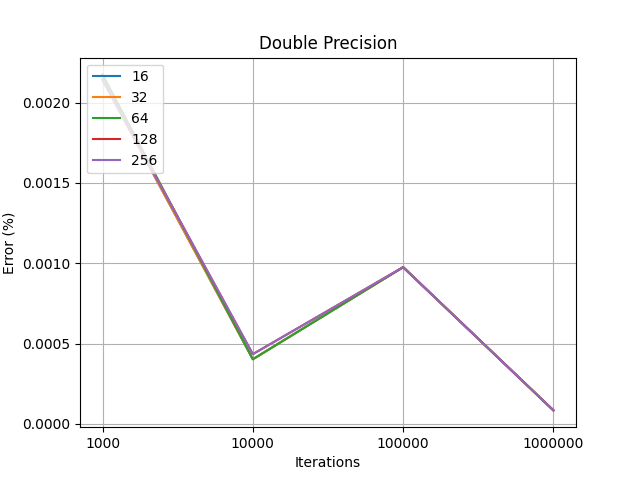
\includegraphics[width=1\linewidth]{graphs/ex_bonus_double_error.png}
%    \caption{Double Precision}
%    \label{fig:ex-single-double-error}
%  \end{subfigure}%
%  \begin{subfigure}{.5\textwidth}
%    \centering
%    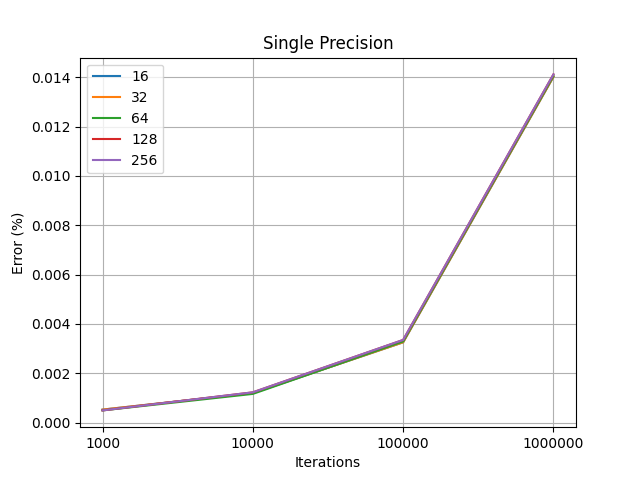
\includegraphics[width=1\linewidth]{graphs/ex_bonus_single_error.png}
%    \caption{Single Precision}
%    \label{fig:ex-bonus-single-error}
%  \end{subfigure}
%  \caption{Graphs of error using double and single precision with different amounts of iterations and block sizes.}
%  \label{fig:fig:ex-bonus-error}
%\end{figure}